\section{Simulations}

Our experiments apply feedback alignment algorithm to network training on both synthetic and real-world data, where a range of networks with different activation functions and levels of regularization are considered. In particular, we compare the regularized feedback alignment (\cref{algo:fa-reg}) with its non-regularized counterpart (\cref{algo:fa}) on two-layer networks. We also evaluate the regularized feedback alignment procedure with two-layer classification networks on \texttt{MNIST} dataset.

\paragraph{Feedback alignment on synthetic dataset.}

For two-layer linear networks, the synthetic data for training are drawn from random linear models, where data $x_i$'s are independently generated and have independent standard Gaussian entries. The model parameter $\zeta\in\Rd$ is also independently generated with standard Gaussian entries, and the training label $y_i$ corresponding to $x_i$ is given by $y_i = x_i\transpose \zeta$. In our experiments, each time $n = 50$ data-label pairs $(x_i,y_i)$ are sampled from a random linear model with dimension $d = 150$, which forms one training dataset $(X,y)$ by stacking them as row vectors.

For two-layer non-linear networks, the generation process of training datasets is customized for different networks following the notion of a teacher-student model. If we deem the network to be trained as a student model, its training dataset is generated by a corresponding teacher model that is an independent and randomly initialized network of the same size and architecture. For each network $f$, its training data $x_i$'s are generated as independent Gaussian vectors like in the random linear model, and their corresponding labels are generated as the outputs of a two-layer network $y_i = f'(x_i)$, where $f'$ is an independent replica of $f$ with random Gaussian first- and second-layer weights. More specifically, if $f$ is a network with ReLU activation and hidden layer width $p$, then $f'$ is also a network with ReLU activation and hidden layer width $p$. In our experiments, all the training datasets $(X,y)$ consist of $n = 50$ training samples with dimension $d = 150$ and the training labels generated from an independent replica of the corresponding network.

\begin{figure}[h]
\centering
\begin{subfigure}[b]{.33\textwidth}
  \centering
  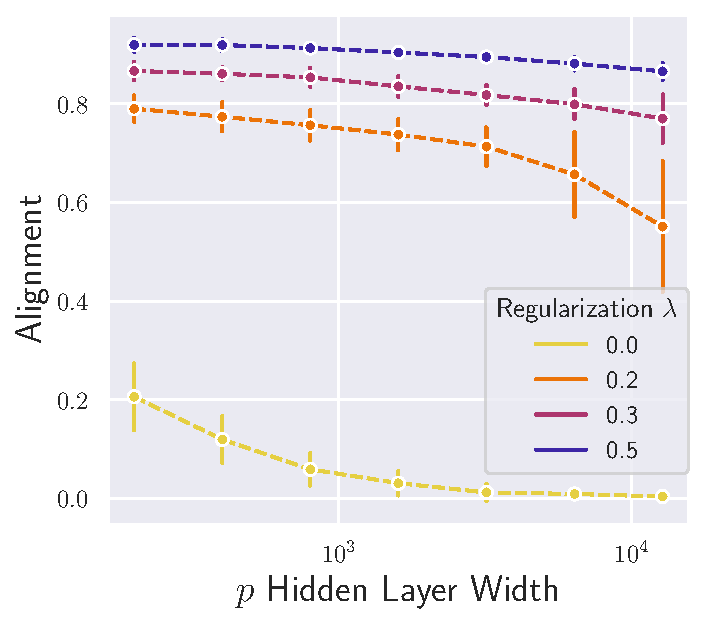
\includegraphics[width=\linewidth]{figures/df_lr_non_autograd_l2_v6.pdf}
  \caption{Alignment on linear network.}
  \label{fig:align_lr_non_autograd_l2}
\end{subfigure}\hfill
\begin{subfigure}[b]{.33\textwidth}
  \centering
  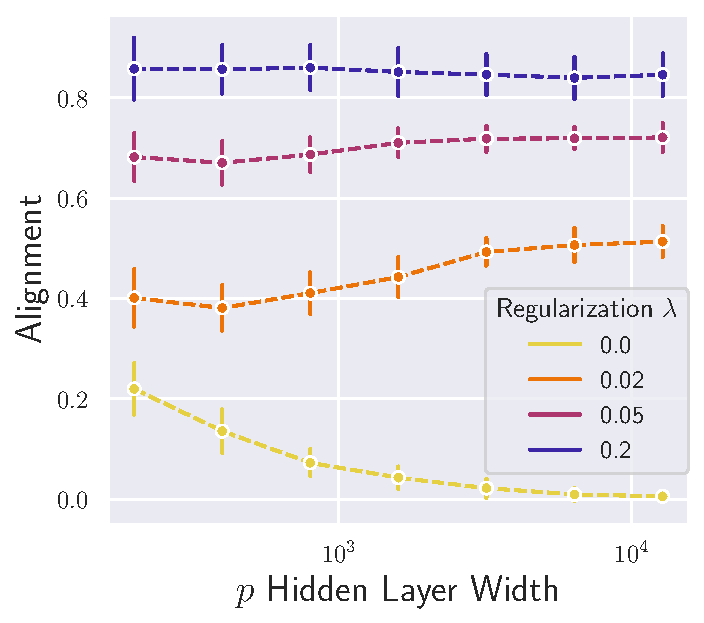
\includegraphics[width=\linewidth]{figures/df_nn_relu_autograd_l2_v6.pdf}
  \caption{Alignment on ReLU network.}
  \label{fig:align_nn_relu_autograd_l2}
\end{subfigure}\hfill
\begin{subfigure}[b]{.33\textwidth}
  \centering
  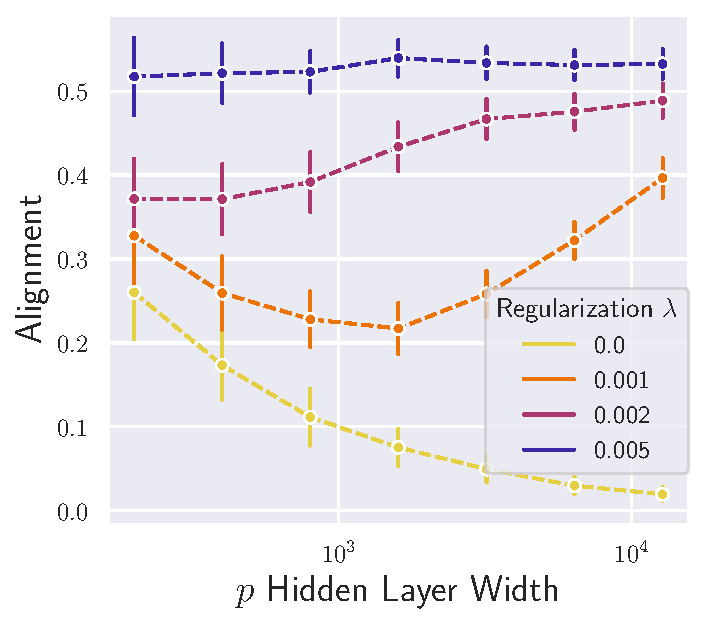
\includegraphics[width=\linewidth]{figures/df_nn_tanh_autograd_l2_v6.pdf}
  \caption{Alignment on Tanh network.}
  \label{fig:align_nn_tanh_autograd_l2}
\end{subfigure}
\medskip
\begin{subfigure}[b]{.33\textwidth}
  \centering
  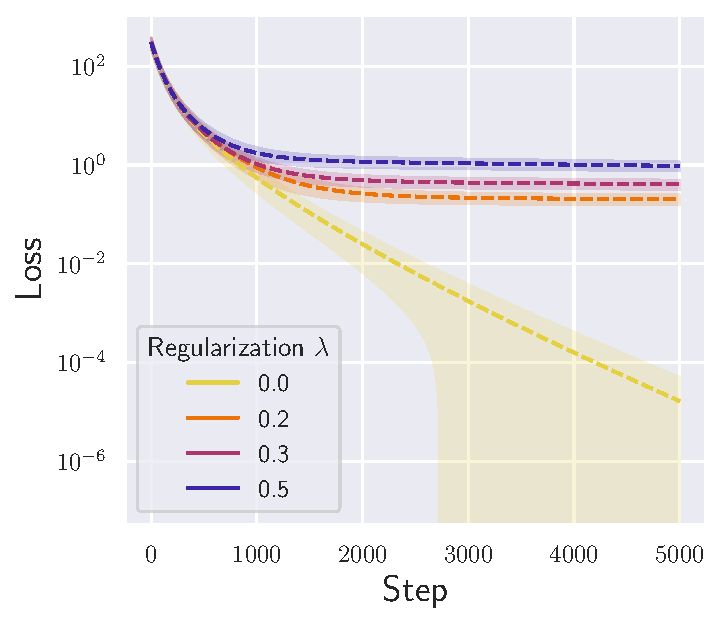
\includegraphics[width=\linewidth]{figures/loss_lr_non_autograd_l2_v1.pdf}
  \caption{Loss on linear network.}
  \label{fig:loss_lr_non_autograd_l2}
\end{subfigure}\hfill
\begin{subfigure}[b]{.33\textwidth}
  \centering
  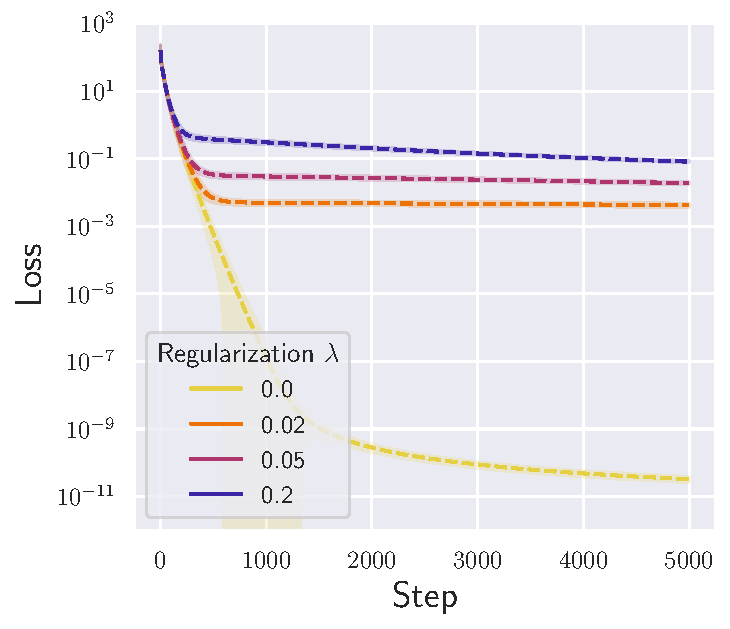
\includegraphics[width=\linewidth]{figures/loss_nn_relu_autograd_l2_v1.pdf}
  \caption{Loss on ReLU network.}
  \label{fig:loss_nn_relu_autograd_l2}
\end{subfigure}\hfill
\begin{subfigure}[b]{.33\textwidth}
  \centering
  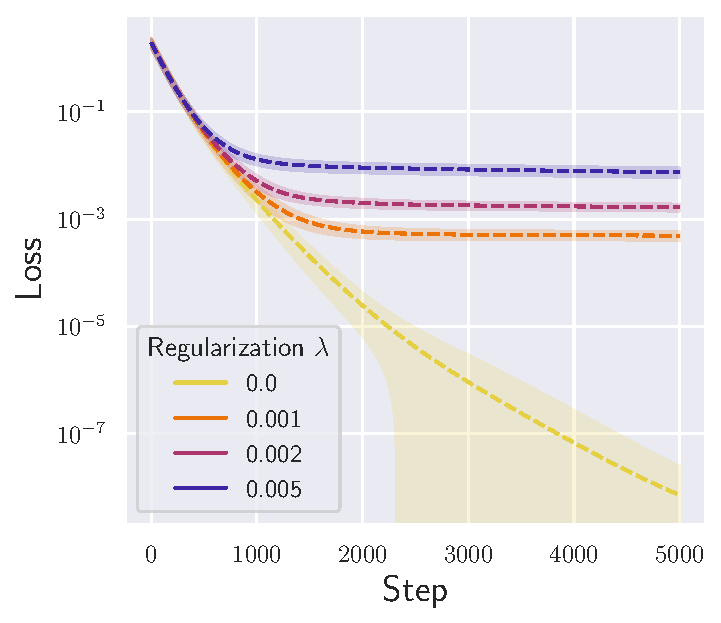
\includegraphics[width=\linewidth]{figures/loss_nn_tanh_autograd_l2_v1.pdf}
  \caption{Loss on Tanh network.}
  \label{fig:loss_nn_tanh_autograd_l2}
\end{subfigure}
\caption{Comparisons on the alignment for feedback alignment algorithm with different levels of $\ell_2$ regularization. In each figure, the $x$-axis denotes the width $p$ of hidden layer, and it is in logarithmic scale; the $y$-axis represents the level of alignment as the normalized inner product between $\beta_t$ and $b$. The data points are the mean value computed across simulations, and the error bars mark the standard deviation among different runs.}
\label{fig:synthetic-l2}
\end{figure}

In \cref{fig:synthetic-l2} we show numerically how alignment depends on regularization and the hidden layer width $p$ when the (regularized) feedback alignment algorithm is applied to two-layer networks with different hidden layer width $p$ and activation $\psi$. In particular, we obtain \cref{fig:align_lr_non_autograd_l2} from performing feedback alignment on linear networks with linear regression data, and \cref{fig:align_nn_relu_autograd_l2,fig:align_nn_tanh_autograd_l2} are the same numerical benchmarks on non-linear networks with ReLU and tanh activation function. For each hidden layer width $p$, we randomly initialize a two-layer network with $p$ hidden neurons and randomly generate a corresponding synthetic dataset for training. Starting from the initialization, we then train the network with feedback alignment algorithm on different levels of regularization and record the alignment between feed-forward weights $\beta$ and backward weights $b$ after the loss converges. For linear networks, we take step size $\eta = 10^{-4}$; for ReLU and Tanh networks, we take $\eta = 10^{-3},10^{-2}$ respectively. This procedure is repeated $50$ times for each $p$, and the simulation results are summarized by their mean and standard deviation. For all three types of networks, the level of alignment converges to zero when the hidden layer width $p$ goes to infinity for feedback alignment algorithm without regularization, while the level of alignment is always kept away from zero for regularized feedback alignment. Further, alignment grows along with the level of regularization $\lambda$ for the same network. Such numerical results strongly support our theoretical statements.

We would like to remark that dropout, a commonly used training technique, as a form of regularization can also help the alignment between forward and backward weights when used together with feedback alignment algorithm \citep{wager2013dropout}. To the best of our knowledge, there is no satisfying theoretical result available that could explain the underlying mechanism.


\paragraph{Feedback alignment on MNIST dataset.}

The training set of \texttt{MNIST} data consists of $6000$ black-and-white images of handwritten digits with dimension $28$ by $28$, and we reshape each of them into an one-dimensional vector of length $d = 784$. The training data $x_i$'s are obtained after normalizing the vectors by their mean and standard deviation. The test dataset with $1000$ samples can be similarly processed. We remark that the structure of the two-layer ReLU network we use for classification has a different output size compared to \eqref{eqn:nonlinear-network}. In particular, the output dimension for \texttt{MNIST} classification is $10$ instead of $1$, and we utilize cross-entropy loss on evaluating the predictions against the categorical labels $y$. During training, we choose a batch size $n = 600$ and there are $100$ steps taken within each epoch with step size $\eta = 10^{-2}$. The training procedure takes $300$ epochs in total. 

\cref{fig:mnist} shows the performance of (regularized) feedback alignment under regularization $\lambda = 0, 0.1, 0.3$. The figure on the right-hand side shows the change on test accuracy for different classifiers during training, and the networks trained with regularization are able to outperform the one without regularization. The regularized feedback alignment quickly converges to the maximum accuracy for larger regularization $\lambda$. In the first two figures, we show the development of alignment during feedback alignment training procedure, and it grows faster with larger regularization. Recall that the second layer weights $\beta\in\RR^{p\times 10}$ is not a vector, and under such scenario the definition of alignment between backpropagated error signals $\dfa$ and $\dbp$ is no longer equivalent to that in \cref{def:alignment}. The first plot follows the definition from \citep{lillicrap2016random} and the second one follows \cref{def:alignment}, and it turns out they are very close to each other numerically.

\begin{figure}[t]
  \centering
  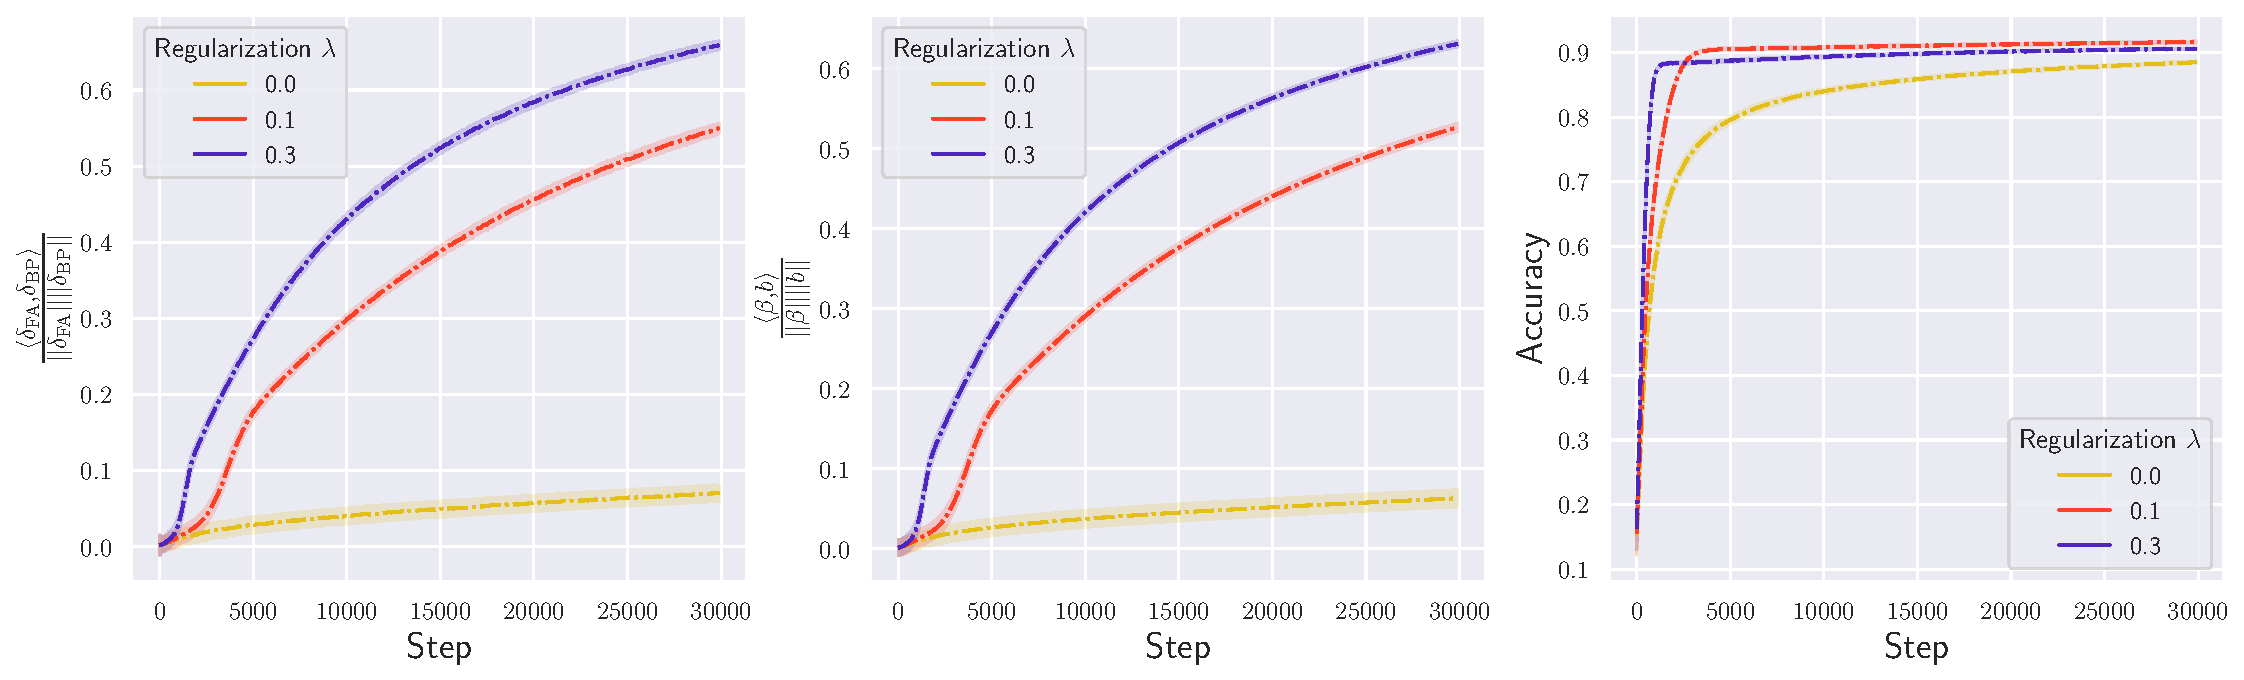
\includegraphics[width=\textwidth]{figures/mnist_2l_v6_horizontal.pdf}
  \caption{Comparisons on alignment and accuracy for feedback alignment algorithm with different levels of $\ell_2$ regularization. In each of the three plots, the $x$-axis represents the number of updates on model parameters. In particular, the $y$-axes in the left and the middle plots show two notions of alignment: alignment of backpropagated error signals and alignment of forward and backward weights, respectively. The plot on the right shows the accuracy achieved by networks on test dataset. The dashed lines and corresponding shaded areas represent the means and the standard deviations over $10$ runs with random initialization.}
  \label{fig:mnist}
\end{figure}